\begin{figure}
\centering
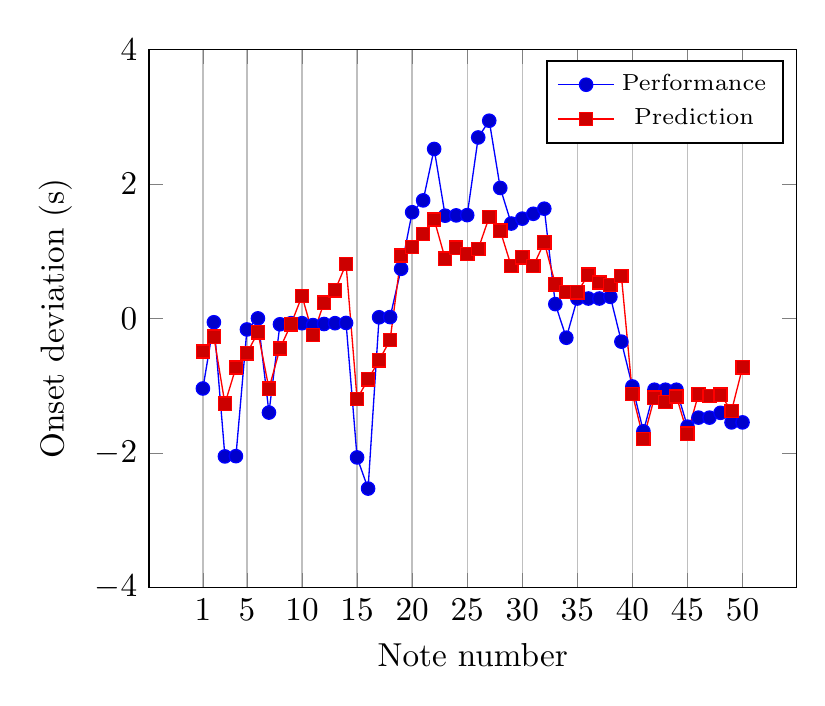
\begin{tikzpicture}[scale=1.2]

\begin{axis}[legend style={font=\scriptsize},
		ylabel={Onset deviation (s)},
        xlabel={Note number},
        ymin=-4, ymax=4,
        xtick={1,5,10,15,20,25,30,35,40,45,50},
        xmajorgrids]

    \addplot coordinates {(1,-1.042) (2,-0.057) (3,-2.052) (4,-2.048) (5,-0.164) (6,0.001) (7,-1.4) (8,-0.087) (9,-0.071) (10,-0.071) (11,-0.099) (12,-0.083) (13,-0.071) (14,-0.067) (15,-2.067) (16,-2.53) (17,0.017) (18,0.02) (19,0.738) (20,1.579) (21,1.755) (22,2.52) (23,1.528) (24,1.532) (25,1.536) (26,2.691) (27,2.94) (28,1.94) (29,1.411) (30,1.484) (31,1.556) (32,1.632) (33,0.213) (34,-0.287) (35,0.296) (36,0.296) (37,0.296) (38,0.321) (39,-0.345) (40,-1.012) (41,-1.679) (42,-1.06) (43,-1.06) (44,-1.06) (45,-1.609) (46,-1.475) (47,-1.475) (48,-1.404) (49,-1.546) (50,-1.546)};
    
     \addlegendentry{Performance}
    
    \addplot coordinates {(1,-0.492) (2,-0.273) (3,-1.267) (4,-0.73) (5,-0.519) (6,-0.206) (7,-1.043) (8,-0.447) (9,-0.087) (10,0.334) (11,-0.245) (12,0.233) (13,0.418) (14,0.809) (15,-1.197) (16,-0.906) (17,-0.624) (18,-0.321) (19,0.936) (20,1.06) (21,1.256) (22,1.471) (23,0.889) (24,1.054) (25,0.957) (26,1.032) (27,1.508) (28,1.304) (29,0.778) (30,0.91) (31,0.778) (32,1.132) (33,0.508) (34,0.393) (35,0.388) (36,0.652) (37,0.534) (38,0.496) (39,0.633) (40,-1.123) (41,-1.791) (42,-1.177) (43,-1.242) (44,-1.161) (45,-1.712) (46,-1.129) (47,-1.151) (48,-1.135) (49,-1.374) (50,-0.728)};
  
   \addlegendentry{Prediction}

\end{axis}
\end{tikzpicture}

\caption[Onset deviation in performance and prediction]{Onset deviation in performance and prediction}
\label{fig:onset}
\end{figure}